
\documentclass[11pt]{article}

\usepackage{common}
\usepackage{subfig}
\title{HW3: Language Modeling}
\author{Jeffrey Ling \\ jling@college.harvard.edu \and Rohil Prasad \\ prasad01@college.harvard.edu }
\begin{document}

\maketitle{}
\section{Introduction}

In this assignment, we examine the problem of language modeling. Given a set of words, we want to determine which word comes after it. Note, however, that there may not be a ``best'' word to follow a prefix. For example, ``fish'' and ``chicken'' could both be almost equally likely to follow the prefix ``I ate \_\_\_''. Therefore, it makes more sense to try and find a good \textbf{probability distribution} of the next word given the prefix. We will define what it means to be ``good'' later on. 

We implement and discuss several different methods of language modeling on the Penn Treebank in this paper. Our first class of algorithms are probabilistic count-based algorithms, consisting of maximum likelihood estimation, Laplace smoothing, Witten-Bell smoothing, and Kneser-Ney smoothing. Our second class of algorithms are deep-learning algorithms, consisting of the neural network described in [Bengio]. Furthermore, we train the neural net with noise contrastive estimation (NCE), a more efficient method for learning the model.

In Section 2, we give a formal description of our problem and establish our notation. In Section 3, we give detailed descriptions of the algorithms listed above. In Section 4, we present our experimental results. In Section 5, we discuss our findings. 

\section{Problem Description}

Assume our training corpus consists of a sequence of words $w_1, w_2, \dots, w_N$ where $w_i$ is drawn from a vocabulary $\mathcal{V}$ for every $i$. Note that for start and end of sentence, we include the tokens \texttt{<s>} and \texttt{</s>}.

While in an ideal situation, we would use the entire history of words $w_1, \ldots, w_{i-1}$ as features to predict word $w_i$, the variable length of such a data representation makes it difficult to handle. Thus, our training data represents this corpus as a context $\mathbf{x}_i$ preceding word $y_i$, where $\mathbf{x}_i$ is the prefix $w_{i-c}w_{i-c+1}\dots w_{i-1}$ of length $c$ and $y_i$ is the suffix $w_i$. 

Our goal is to train a model that will take in an input sequence $\mathbf{x}$ of words and output a vector of probabilities $\mathbf{y} \in \mathbb{R}^{|\mathcal{V}|}$ where $\mathbf{y}_i = p(v_i | \mathbf{x})$ for $v_i$ the $i$th word of $\mathcal{V}$.

\subsection{Count-Based Model Notation}

We use some specific notation for our count-based models. 
\begin{itemize}
  \item $w^{i-1}_{i-n+1}$, the context, is our shorthand for the size $n-1$ prefix $w_{i-n+1}w_{i-n+2}\dots w_{i-1}$ before $w_i$. When $n = 2$, we will continue to use $w_{i-1}$. 
  \item $c(w_i)$ denotes the total number of occurrences of the word $w_i$ in the training corpus. 
  \item $c(w^{i-1}_{i-n+1}, w_i)$ denotes the total number of occurrences of the word $w_i$ after the prefix $w^{i-1}_{i-n+1}$ in the training corpus. 
  \item $N(\cdot, w_i)$ denotes the total number of unique prefixes of size $n$ that $w_i$ has in the training corpus. 
  \item $N(w^{i-1}_{i-n+1}, \cdot)$ denotes the total number of unique suffixes that the sequence $w^{i-1}_{i-n+1}$ has in the training corpus. 
\end{itemize}

\subsection{Evaluation}

Because there are multiple possible ``correct'' words that follow a specific context, it does not make sense to use percent accuracy as a metric. Instead, we use the probability distribution predicted over words and compute the perplexity, a metric derived from the negative log-likelihood (NLL).

Specifically, the NLL is given over the data as
$$NLL = -\sum_{i=1}^N \log p(w_i | w_{i-1}, \ldots, w_1)$$
and the perplexity
$$PPL = \exp(NLL)$$

\section{Model and Algorithms}

\subsection{Count-Based Models}

All of our count-based models are $n$-gram models, meaning we fix an $n$ and assume $p(w_i|w^{i-1}_1) = p(w_i|w^{i-1}_{i-n+1})$. 

\subsubsection{Maximum Likelihood Estimation}

The maximum likelihood estimation $p_{MLE}(w_i|w^{i-1}_{i-n+1})$ is given by 
$$p_{MLE}(w_i|w^{i-1}_{i-n+1}) = \frac{c(w^{i-1}_{i-n+1}, w_i)}{\sum_{w' \in \mathcal{V}} c(w^{i-1}_{i-n+1}, w')}$$

This is by definition the probability over the training corpus of the word $w_i$ appearing conditioned on the prefix being equal to $w^{i-1}_{i-n+1}$. 

\subsubsection{Laplace Smoothing}

 One thing to note is that our MLE model will by definition assign a (clearly erroneous) probability of $0$ to $p(w|w^{i-1}_{i-n+1})$ for any sequence $w_i, w^{i-1}_{i-n+1}$ that does not appear in the training corpus. This poses a problem for larger $n$, since the number of distinct $n$-grams in the training corpus will only form a small fraction of the number $|\mathcal{V}|^n$ of possible $n$-grams.

We fix this by adding $\alpha$ to the count of every word. Then, our probability becomes 
$$p_L(w_i|w^{i-1}_{i-n+1}, \alpha) = \frac{\alpha + c(w^{i-1}_{i-n+1}, w_i)}{\alpha \cdot |\mathcal{V}| + \sum_{w' \in \mathcal{V}} c(w^{i-1}_{i-n+1}, w')}$$

In our experiments, we set $\alpha = 0.01$. 

\subsubsection{Witten-Bell Smoothing}

Witten-Bell smoothing relies on the idea of interpolation. In order to predict word $w_i$ from context $w_{i-n+1}^{i-1}$, instead of only using trigrams or bigrams, we take a weighted average of the probabilities together with the unigram probabilities (i.e. the frequency of $w_i$ in the training corpus).

Specifically, The Witten-Bell probability for bigrams with an additive smoothing parameter $\alpha$ is written as

$$p_{WB}(w_i|w_{i-1}) = \lambda_{w_{i-1}} p_L(w_i|w_{i-1}, \alpha) + (1-\lambda_{w_{i-1}}) p_L(w_i| \alpha)$$

where $\lambda_{w_{i-1}}$ is determined by the following equation:

$$1 - \lambda_{w_{i-1}} = \frac{N(w_{i-1}, \cdot)}{N(w_{i-1}, \cdot) + c(w_{i-1}, w_i)}$$

We can then define Witten-Bell recursively for $n$-grams as

$$p_{WB}(w_i|w^{i-1}_{i-n+1}) = \lambda_{w^{i-1}_{i-n+1}} p_L(w_i|w^{i-1}_{i-n+1}, \alpha) + (1-\lambda_{w^{i-1}_{i-n+1}}) p_{WB}(w_i|w^{i-1}_{i-n+2})$$

where $\lambda_{w^{i-1}_{i-n+1}}$ is given by:

$$1 - \lambda_{w^{i-1}_{i-n+1}} = \frac{N(w^{i-1}_{i-n+1}, \cdot)}{N(w^{i-1}_{i-n+1}, \cdot) + c(w_i, w^{i-1}_{i-n+1})}$$ 

\subsubsection{Kneser-Ney Smoothing}

For Kneser-Ney, we define the lower-order probabilities as follows. Fix a ``discount parameter'' $\delta$. For unigrams, the equation is:

$$p_{KN}(w_i) = N(\cdot, w_i)/\sum_{w' \in \mathcal{V}} N(\cdot, w')$$

Then for bigrams, it is defined as 

$$p_{KN}(w_i | w_{i-1}) = \frac{\text{max}(c(w_{i-1}, w_i) - \delta, 0)}{\sum_{w' \in \mathcal{V}} c(w_{i-1}, w')}$$

Finally, we can define it recursively for general $n$-grams:

$$p_{KN}(w_i | w^{i-1}_{i-n+1}) = \frac{\text{max}(c(w^{i-1}_{i-n+1}, w_i) - \delta, 0)}{\sum_{w' \in \mathcal{V}}c(w^{i-1}_{i-n+1}, w')}$$

The optimal value for $\delta$ is determined by grid search on a validation set. 

\subsection{Neural Network Model}

The neural network model of Bengio aims to directly learn a function from context $c_i = w_{i-n+1}^{i-1}$ to the word $w_i$. We have parameters
\begin{itemize}
\item $W_0 \in \mathbb{R}^{|\mcV| \times d_{in}}$, a lookup table of word embeddings,
\item $W_1 \in \mathbb{R}^{nd_{in} \times d_{hid}}$, $b_1 \in \mathbb{R}^{d_{hid}}$,
\item $W_2 \in \mathbb{R}^{d_{hid} \times |\mcV|}$, $b_2 \in \mathbb{R}^{|\mcV|}$,
\end{itemize}

First, the context words are transformed into word embeddings with $W_0$ and concatenated to form a vector $ \mathbf{x_0}$ of size $n \cdot  d_{in}$. Then, we get a vector of scores
$$\mathbf{z} = \tanh(\mathbf{x_0}W_1 + b_1)W_2 + b_2 \in \mathbb{R}^{|\mcV|}$$

We can then force a distribution over words by taking the softmax $\widehat{y} = softmax(\mathbf{z})$, where $\widehat{y}_k$ is our predicted probability of word $k$.

\subsection{Noise Contrastive Estimation}

The architecture described above can be difficult to train due to the computational cost of a softmax over the entire vocabulary. Mnih and Teh solve this problem using a slightly different training method, which introduces the binary noise random variable $D$. We thus have a binary classification task that uses pairs $(w_{i-n+1}^{i-1}, w_i)$ from the corpus corresponding to $D = 1$, with $K$ noise words $s_1, \ldots, s_K$ per context (sampled from the unigram distribution $p_{ML}(w)$) giving $(w_{i-n+1}^{i-1}, s_j)$ corresponding to $D = 0$.

We can assume the prior $p(D = 1) = \frac{1}{K+1}$. Using shorthand $x = w_{i-n+1}^{i-1}, y = w_i$, we can then write the probability of a non-noise sample as
\begin{align*}
p(D = 1 | x, y) & = \frac{p(y | D = 1, x)p(D = 1|x)}{p(y | D=0, x)p(D = 0|x) + p(y|D = 1, x)p(D = 1 | x)} \\
& = \frac{p(y | D = 1, x)}{Kp(y | D=0, x) + p(y|D = 1, x)} \\
& = \sigma(\log p(y | D = 1, x) - \log (Kp(y | D = 0, x)))
\end{align*}

Therefore our binary classification log-likelihood is
$$L(\theta) = \sum_i \log \sigma(\log p(w_i | D = 1, x_i) - \log (Kp(w_i | D = 0, x_i))) + $$
$$+\sum_{k=1}^K \log (1 - \sigma(\log p(s_{i,k} | D = 1 , x_i) - \log(Kp(s_{i,k}| D = 0, x))))$$

Note that $p(y | D = 1, x)$ is the probability of a specific word according to our predictive model, and so is a function of the parameters $\theta$. $p(y | D = 0, x)$ is the noise distribution $p_{ML}$. Mnih and Teh find that in practice, replacing $p(y_i | D = 1, x_i)$ with the score $z_{y_i}$ as computed by our model is equally effective for training.

Thus, we have
$$L(\theta) = \sum_i \log \sigma(z_{w_i} - \log (Kp_{ML}(w_i))) + \sum_{k=1}^K \log(1 - \sigma(z_{s_{i,k}} - \log(Kp_{ML}(s_{i,k}))))$$
as our new objective.

To efficiently compute the scores $z_{w}$, instead of taking the full linear product as before, we can take a dot product of $\tanh(\mathbf{x_0}W_1 + b_1)$ with the row of $W_2$ corresponding to $w$.

\section{Experiments}

Our overall best results across our count-based and neural network models are listed here. Note that the MLE models only have a perplexity that makes sense when tested on Train, since they give unseen $n$-grams probabilities of $0$ which yields an undefined perplexity.

\begin{table}[h]
\centering
\begin{tabular}{llccc}
 \toprule
 Model &  & Train & Valid & Blanks\\
 \midrule
 \textsc{MLE (Bigrams)} & & 68 & NA & NA \\
 \textsc{MLE (Trigrams)} & & 8 & NA & NA \\
 \textsc{Laplace (Bigrams)} & & 96 & 297 & 4.59 \\
 \textsc{Laplace (Trigrams)} & & 155 & 399 & 11.86 \\
\textsc{Witten-Bell (Bigrams)} & & 85 & 215 & 3.59 \\
\textsc{Witten-Bell (Trigrams)} & & 24 & 369 & 5.24 \\
 \textsc{Neural (GPU)} & & 233 & 246 & 3.94\\
 \textsc{Neural (NCE)} & & & 252 & 3.73 \\
 \bottomrule
\end{tabular}
\caption{\label{tab:results} Perplexities on PTB language modeling.}
\end{table}

\subsection{Count-Based Models}


For our count-based models, we noticed that the perplexity of Laplace smoothing and Witten-Bell smoothing on our validation set were sensitive to the hyperparameter $\alpha$. Therefore, we did an exhaustive grid-search, running over $\alpha = n \cdot 10^{-k}$ for $1 \leq n \leq 9$ and for several $k$ on our valid.txt validation set. 

We graph perplexity on the validation set for Laplace smoothing and Witten-Bell smoothing for both bigrams and trigrams. 

\begin{figure}
\centering
\subfloat[Bigrams]{ 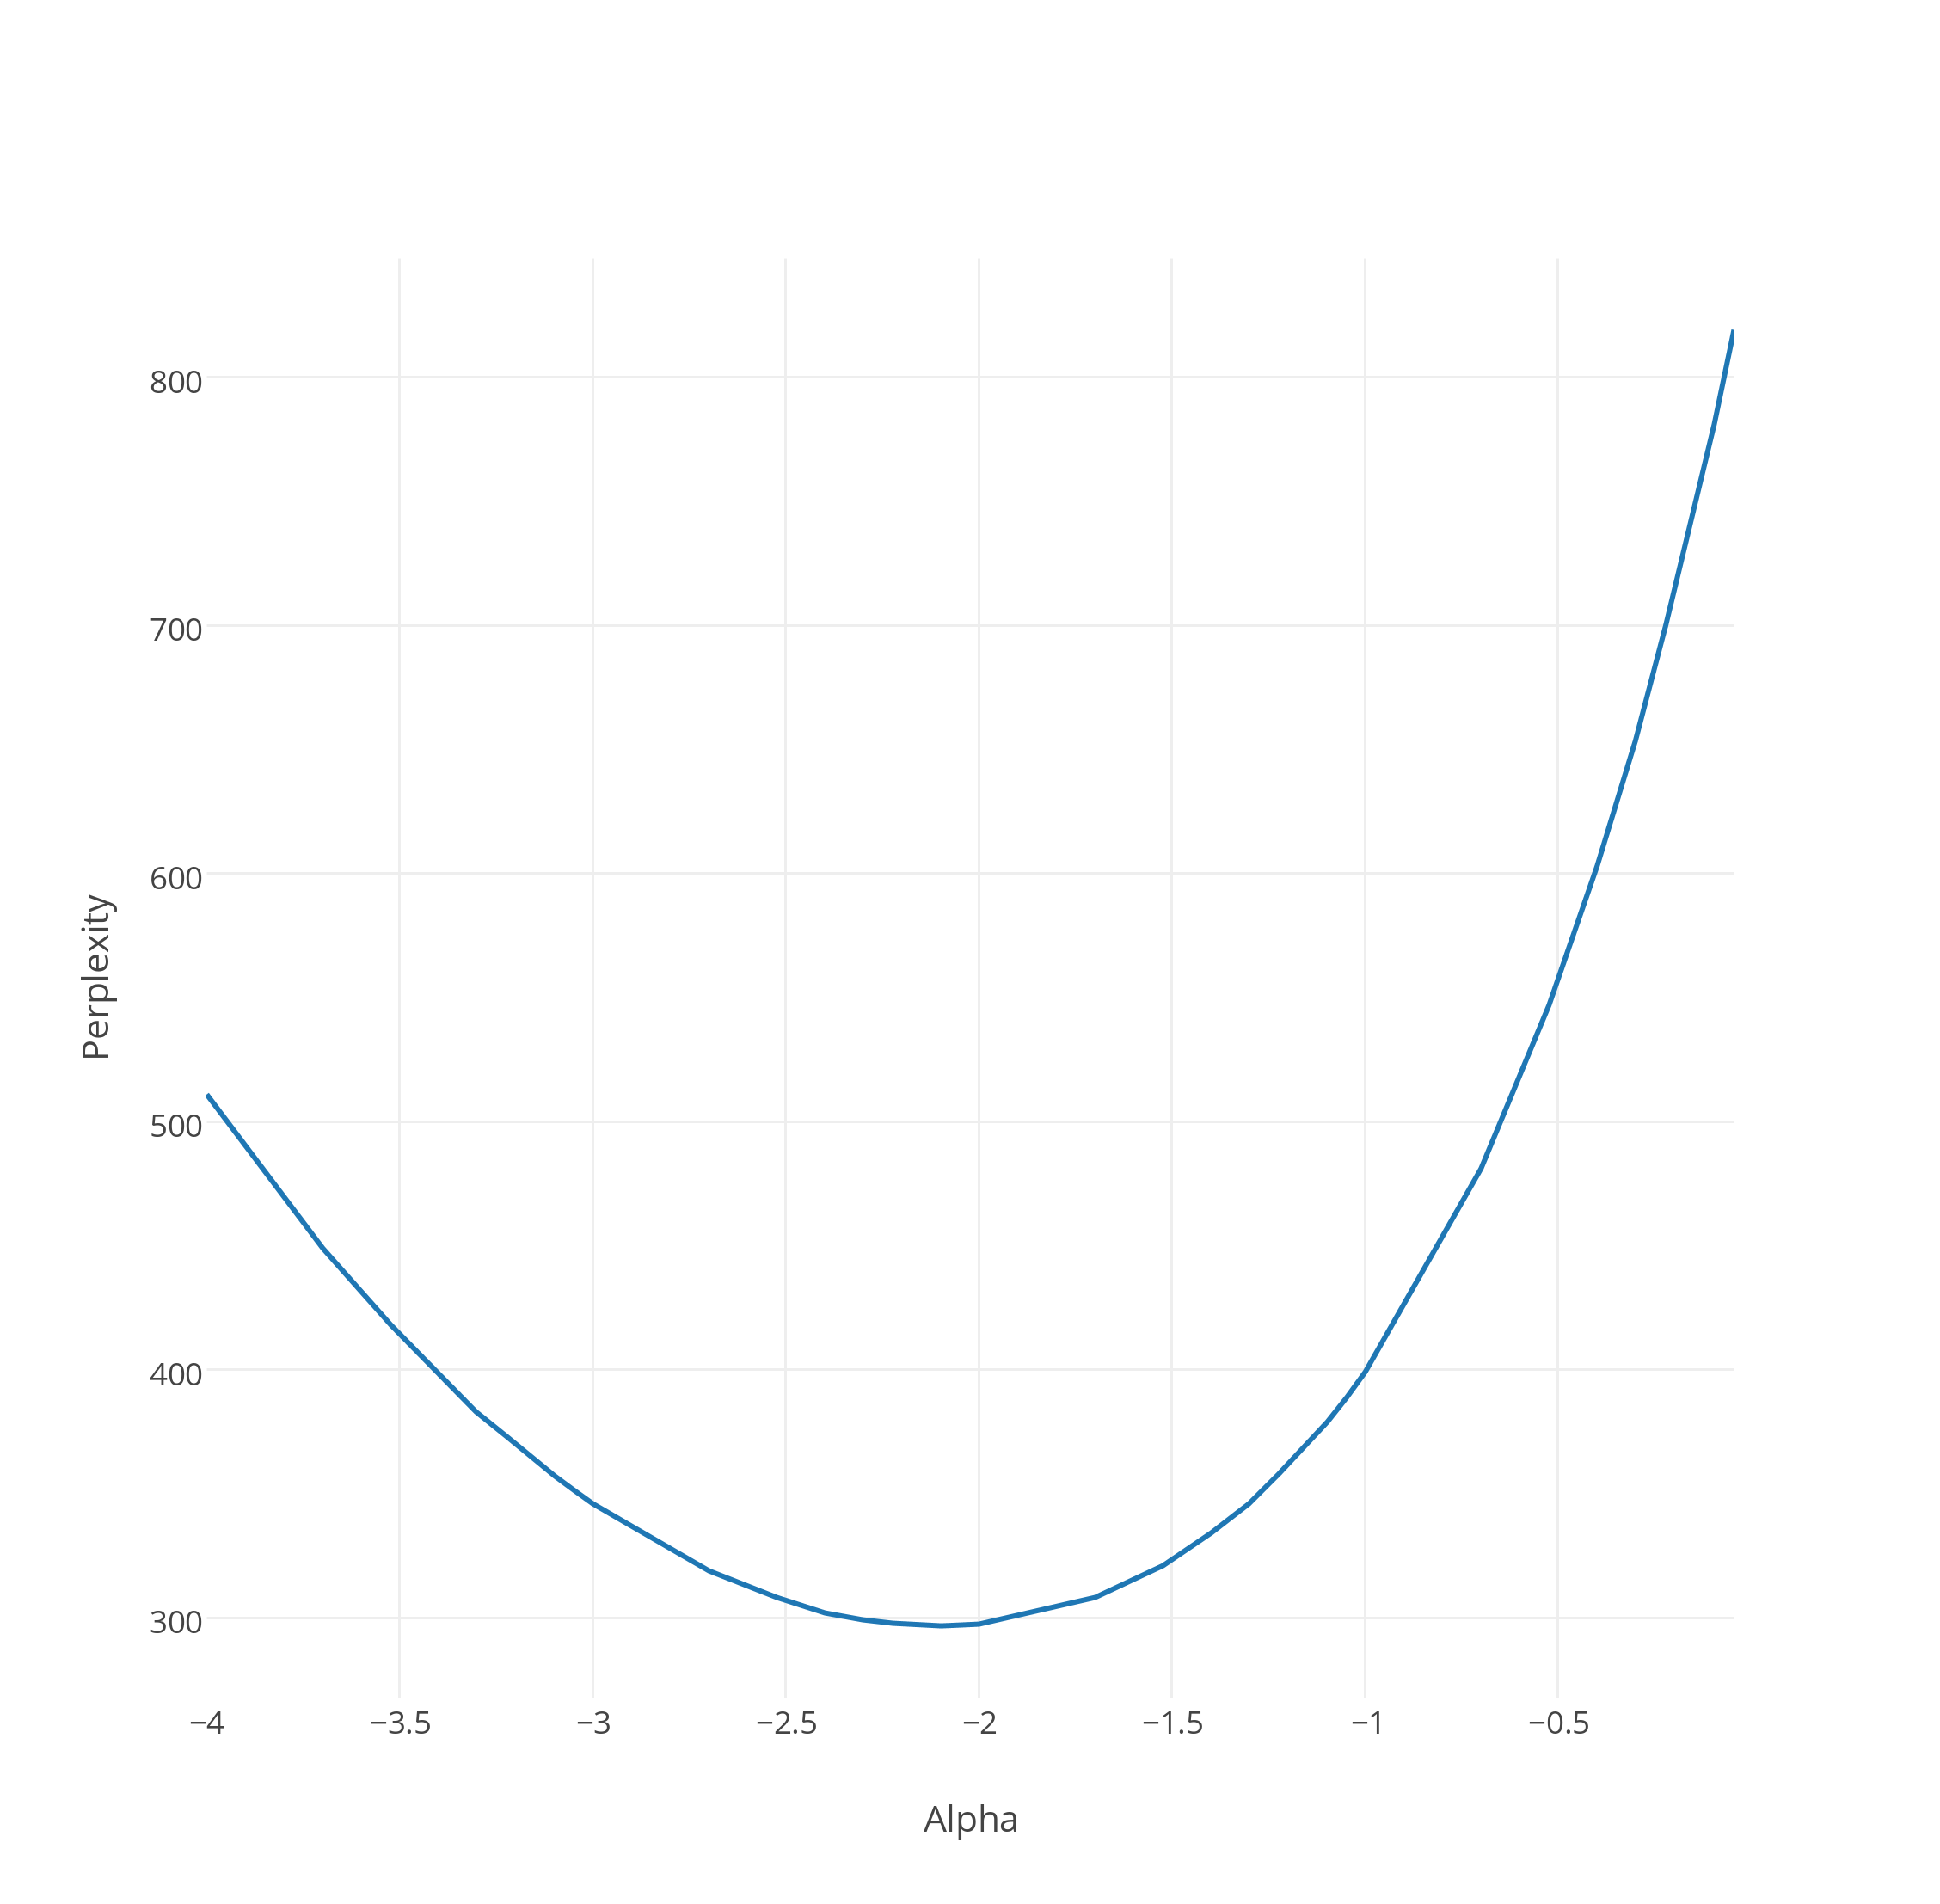
\includegraphics[scale=0.33]{laplace_2grams.png} \label{fig:laplace2} }
\hfill
\subfloat[Trigrams]{ 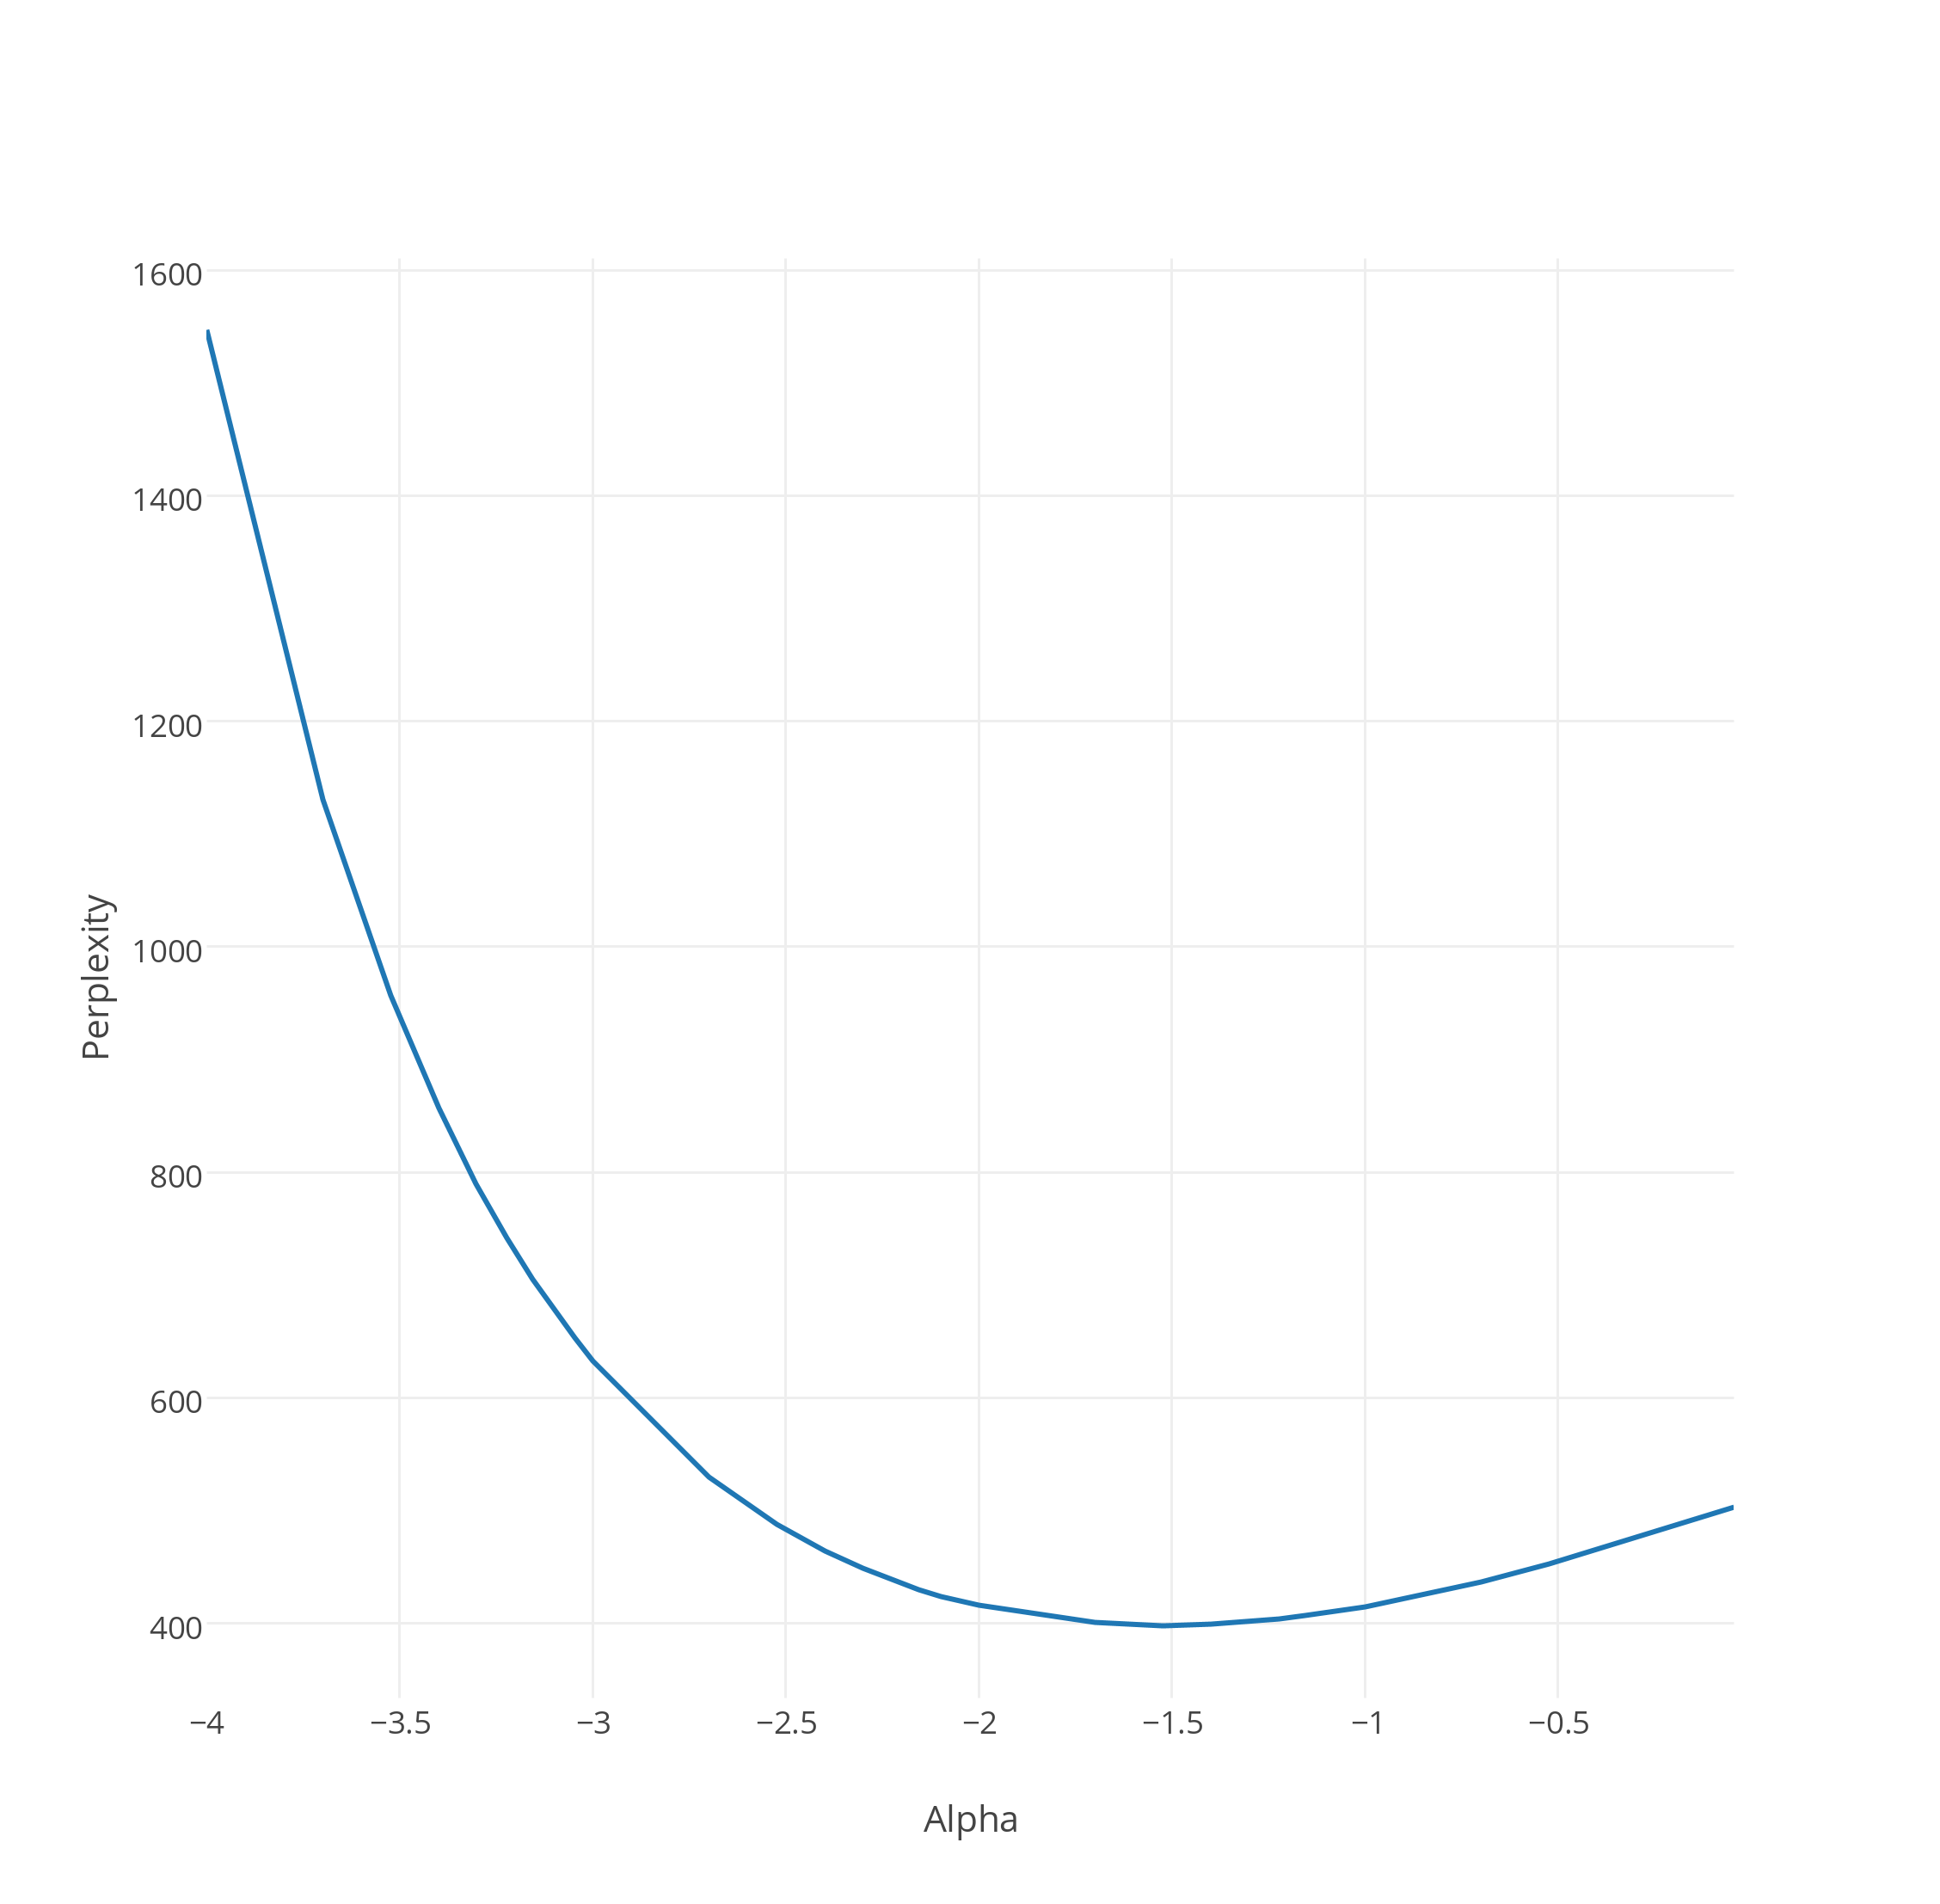
\includegraphics[scale=0.33]{laplace_3grams.png} \label{fig:laplace3} }
\caption{Laplace smoothing.}
\end{figure}

\begin{figure}
\centering
\subfloat[Bigrams]{ 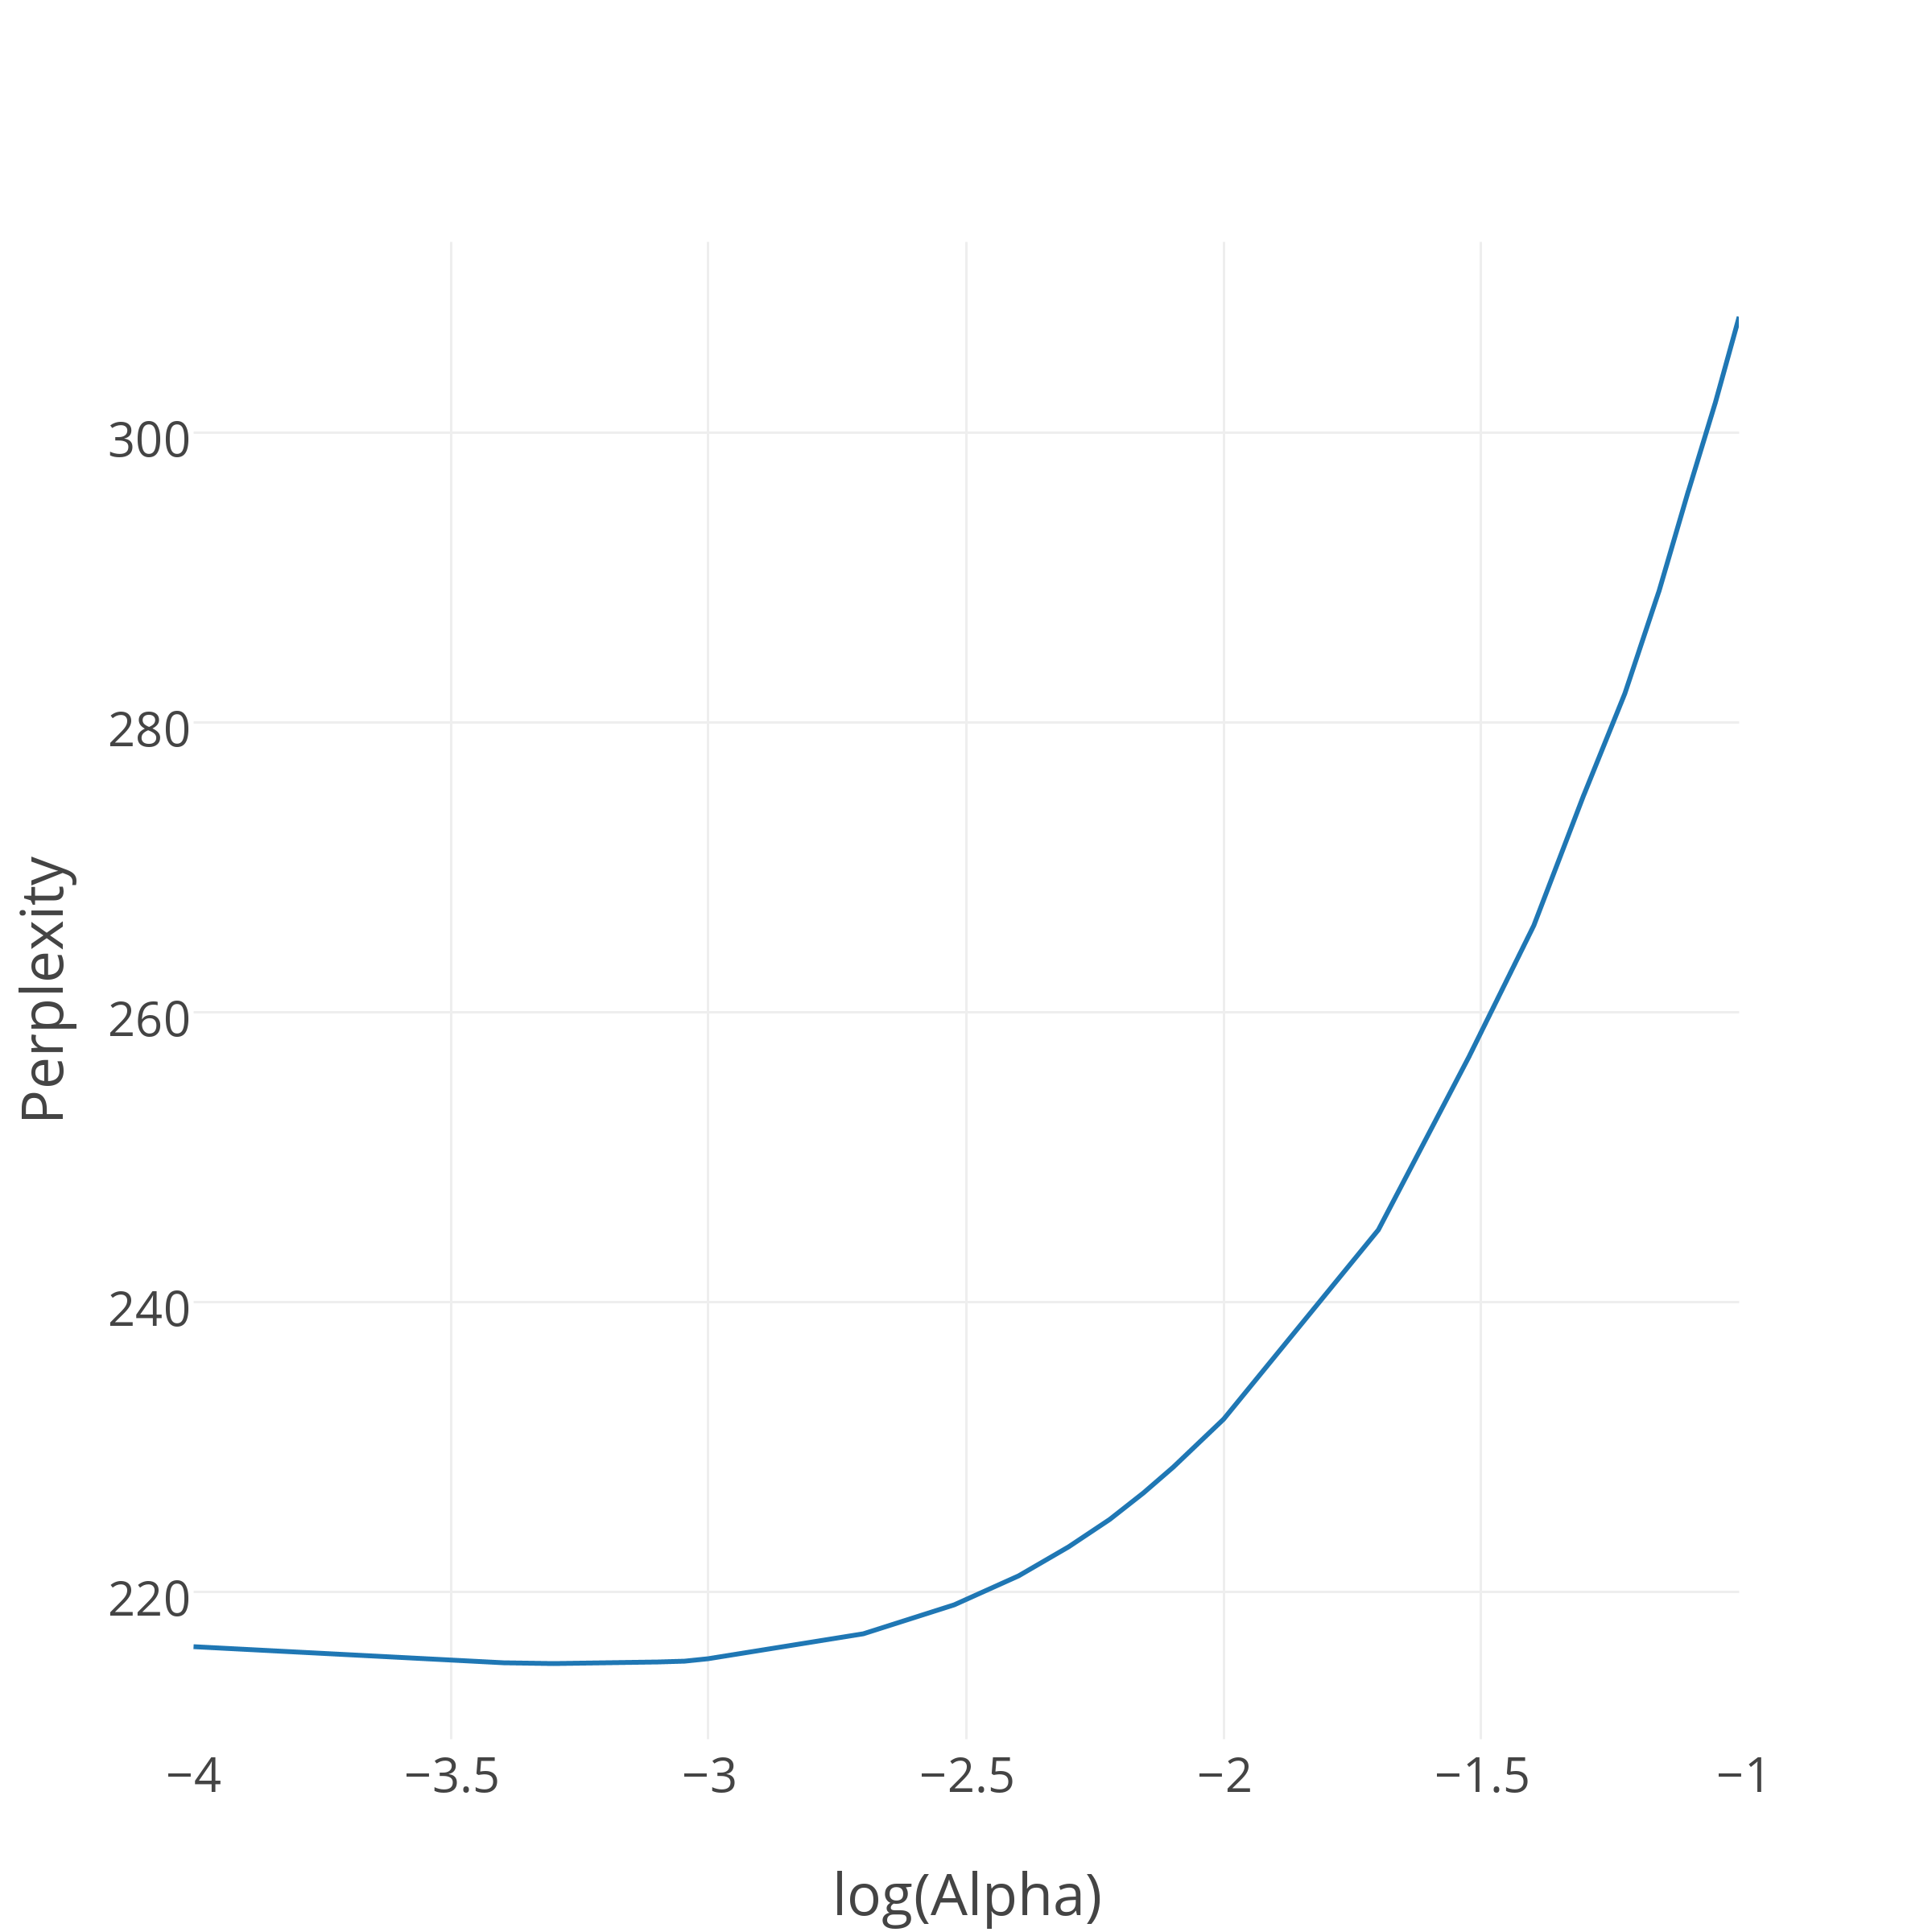
\includegraphics[scale=0.33]{wb_2grams.png} \label{fig:wb2} }
\hfill
\subfloat[Trigrams] {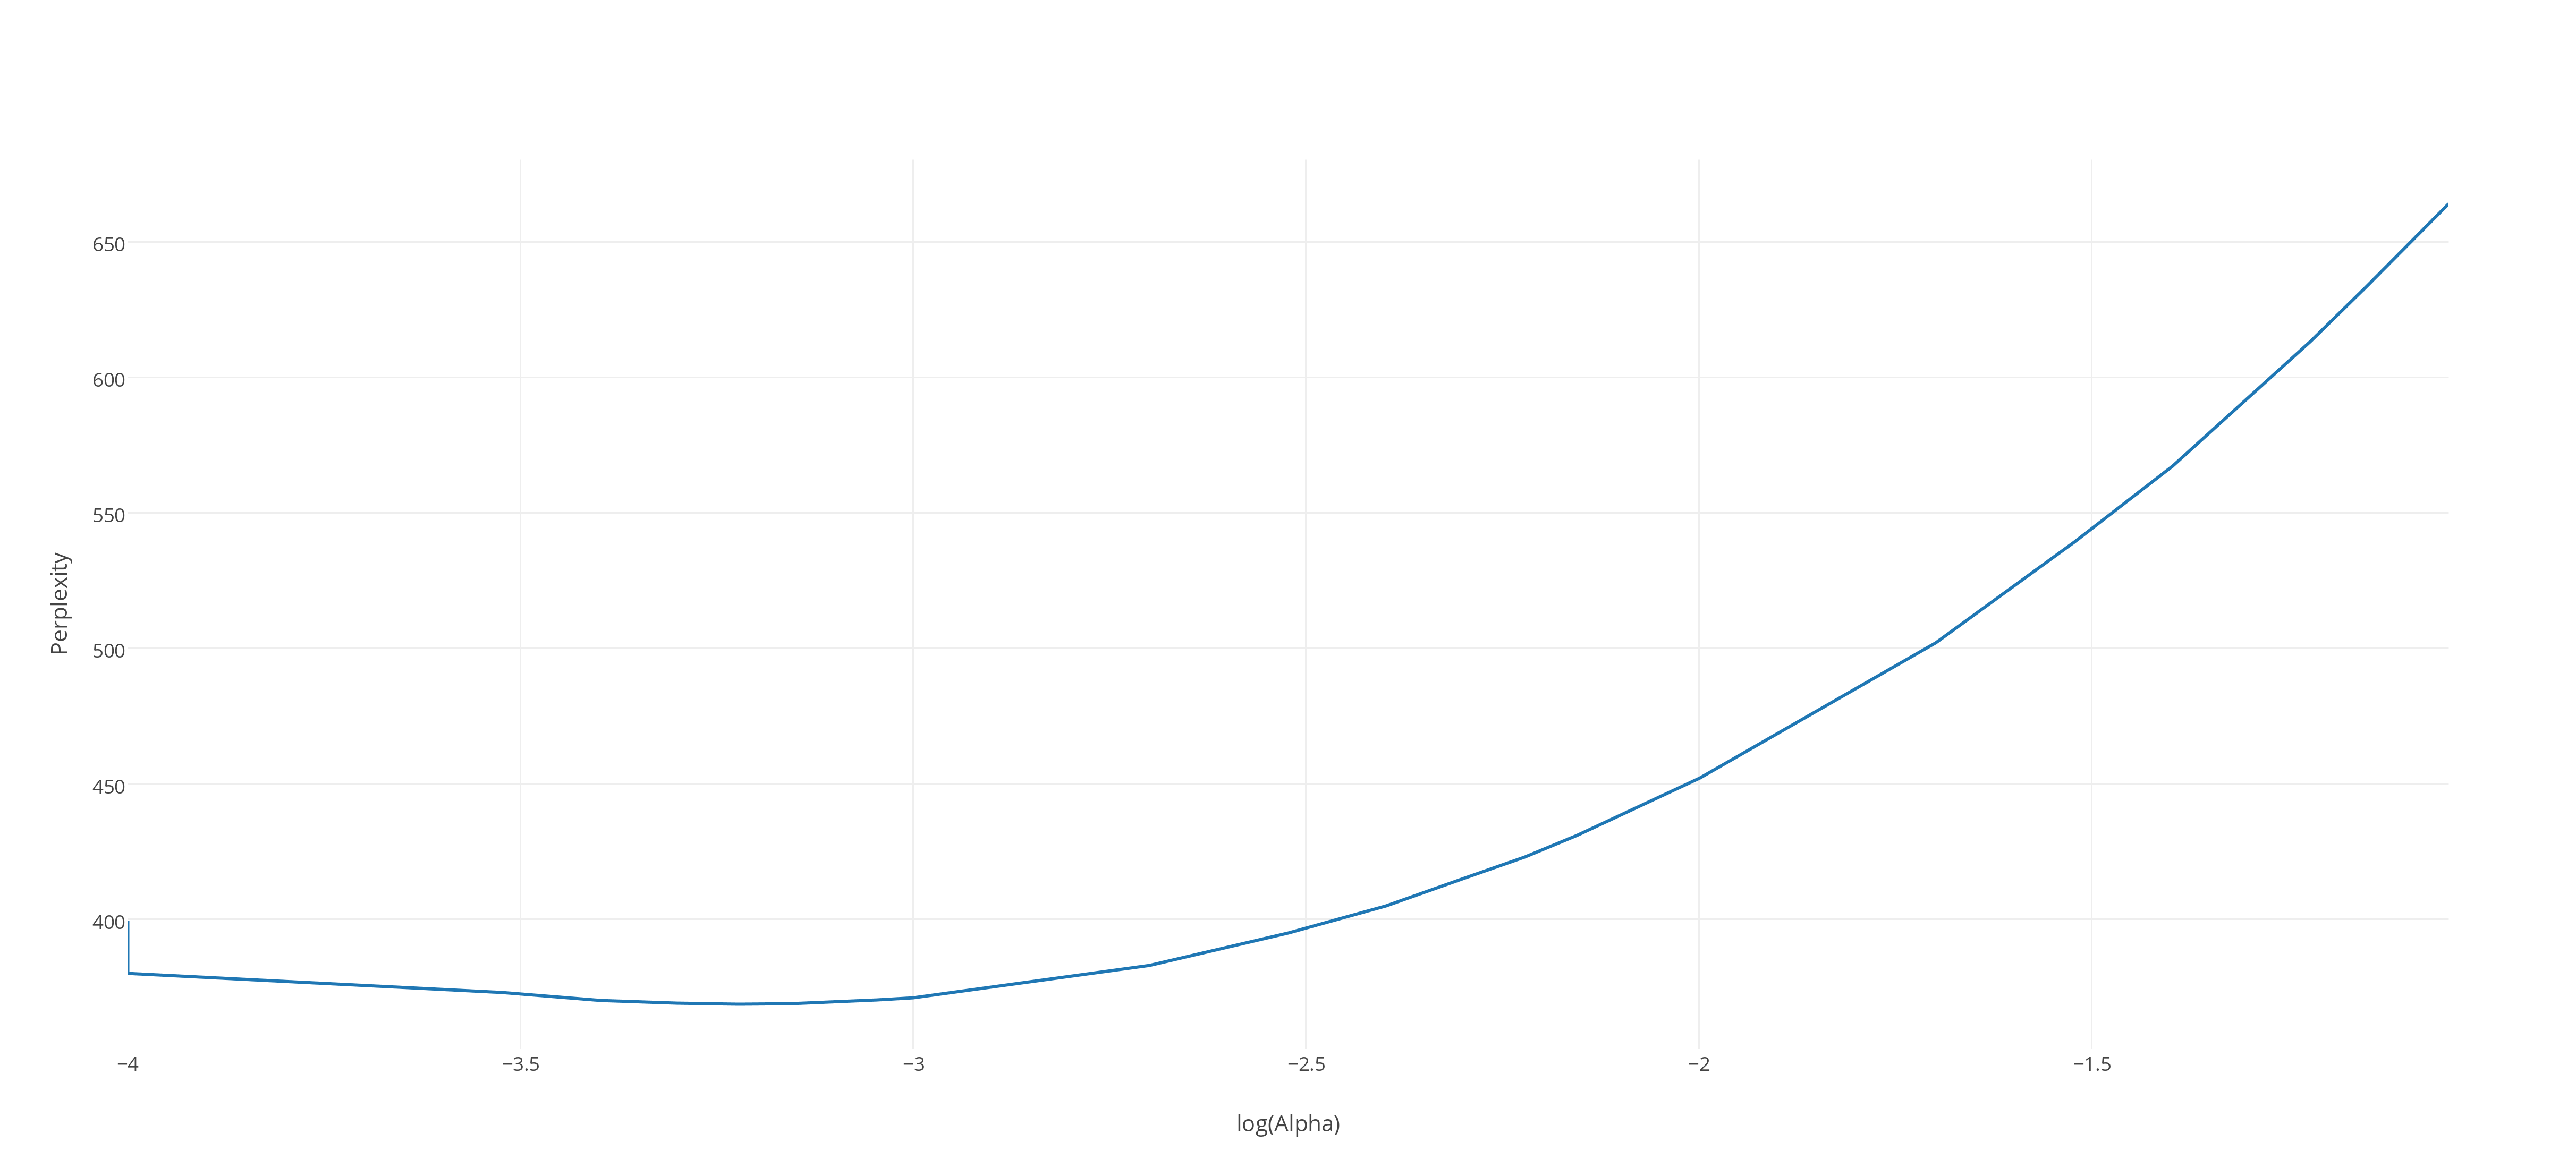
\includegraphics[scale=0.33]{wb_3grams.png}  \label{fig:wb3} }
\caption{Witten-Bell smoothing.}
\end{figure}

Laplace smoothing perplexity is graphed for $\alpha = n \cdot 10^{-k}$ for $k \in \{-4, -3, -2, -1\}$ while Witten-Bell smoothing perplexity is graphed for $\alpha = n \cdot 10^{-k}$ for $k \in \{-4, -3, -2\}$. The data for $k = -1$ is cut off in this case to allow easier visualization, as the perplexity starts to increase very quickly past $\alpha = 0.1$.  

We give the optimal $\alpha$ with their corresponding perplexity in a table below. 

\begin{table}[h]
  \centering
  \begin{tabular}{lccc}
    \toprule
    Model & N-gram Size & $\alpha$ & Perplexity \\
    \midrule
    \textsc{Laplace Smoothing} & 2 & 0.008 & 297 \\
    & 3 & 0.03 & 399 \\
    \textsc{Witten-Bell Smoothing} & 2 & 0.0007 & 215 \\
    & 3 & 0.0006 & 369 \\
    \bottomrule
  \end{tabular}
  \caption{\label{tab:alpha} Best $\alpha$ parameters for count-based models}
\end{table}

\subsection{Neural network models}

We trained using SGD with learning rate $0.01$, batch size 32, and stopped training when perplexity on the validation set stopped decreasing. We used word embedding size $d_{in} = 50$ and hidden layer size $d_{hid} = 100$. The models used a context size of 5 words.

For normal training on the Bengio model, we used GPU. This allowed us to complete an epoch in about 3 minutes. We compute final perplexities for the train, valid, and valid blanks data, which are reported in Table~\ref{tab:results}.

For NCE, we started training with learning rate $10$, since it seemed to not learn properly with small learning rate. After a few iterations we drop the learning rate to $0.01$. We used the same architecture and set the noise parameter $K = 10$. The timing was quite fast, completing an epoch in about 7 minutes on CPU. Final results are reported in Table~\ref{tab:results}.

%% plot learning curves

Unfortunately, the perplexities seem higher than desired, although the results on Kaggle seem mostly consistent. This could be due to a computational error on our evaluation side.

\subsection{Word Embeddings}

%% TODO

\section{Conclusion}

The count-based model results were very surprising. First of all, our Witten-Bell bigram model had lower perplexity than the neural model on the valid set. Second of all, our trigram models universally performed much worse than our bigram models. 

We found that training NCE properly was difficult and ate up hours on this assignment. In the end, the problem was that NCE trains very slowly, so the initial epochs showed wildly high perplexities for small learning rates. Nonetheless, it definitely gets significant speedups compared to training the full model on CPU. 


%\bibliographystyle{apalike}
%\bibliography{writeup}

\end{document}
